For our analysis, we used data from Kickstarter.com hosted on the web crawler platform Webrobots.io. We analyzed 75,810 projects that applied for Kickstarter funding in the time period between June 17, 2021, and May 19, 2022. For every project, we tracked specific project indicators such as project ID, project name, project image, the text blurb (which is taken as the text caption in our project), the current state of the project, goal amount in USD, pledged amount in USD, and industry branch.  The Pie chart below shows the project categories included art, comics, crafts, dance, design, fashion, film and video, food, journalism, music, photography, publishing, technology, and theater. Our primary outcome variable was the fundraising outcome. The data source defined four possible financ-ing outcomes: successful, canceled, failed, and live financing. Successful financing means that the project reached both its financial goal and fundraising deadline (39\% of all projects). Some 58\% of projects failed to amass the goal amount by the fundraising deadline. Five per-cent of projects were canceled prior to the fundraising campaign launch for reasons such as deadlines and/or the financial goal not being realistic. Lastly, 2\% of projects were “Live”, meaning currently in the process of fundraising. Since their final status had yet to be determined, they were excluded from the analysis. We subsumed the canceled and failed projects in the group named “unsuccessful financing”, thus effectively making fundraising outcome a dichotomous variable, i.e., successful and unsuccessful projects. Backers are individuals who pledge money to join creators in bringing projects to life,i.e., to support a cre-ative process. They receive various rewards for their engagement as a creator's way to share a piece of proj-ect with their backer community (Kickstarter, 2021). The more backers a project receives, the more chances it has to hit its goal amount and fundraising deadline. The goal amount is the amount of money creators are setting on Kickstarter.com.  For our analysis, we do not consider the number of backers, goal amount, pledged amount, pledged amount per backer, and pledged to goal ratio. According to Kick-starter.com,once a creator launches their project, the funding goal and deadline are locked in and cannot be changed. The pledged amount represents the amount of money a specific project has received from its backers. Only projects whose pledged amount hits or exceeds their goal amount within a specific deadline will be suc-cessfully financed (Kickstarter, 2021). 

\vspace{-0.5em}
\begin{figure}
  \centering
  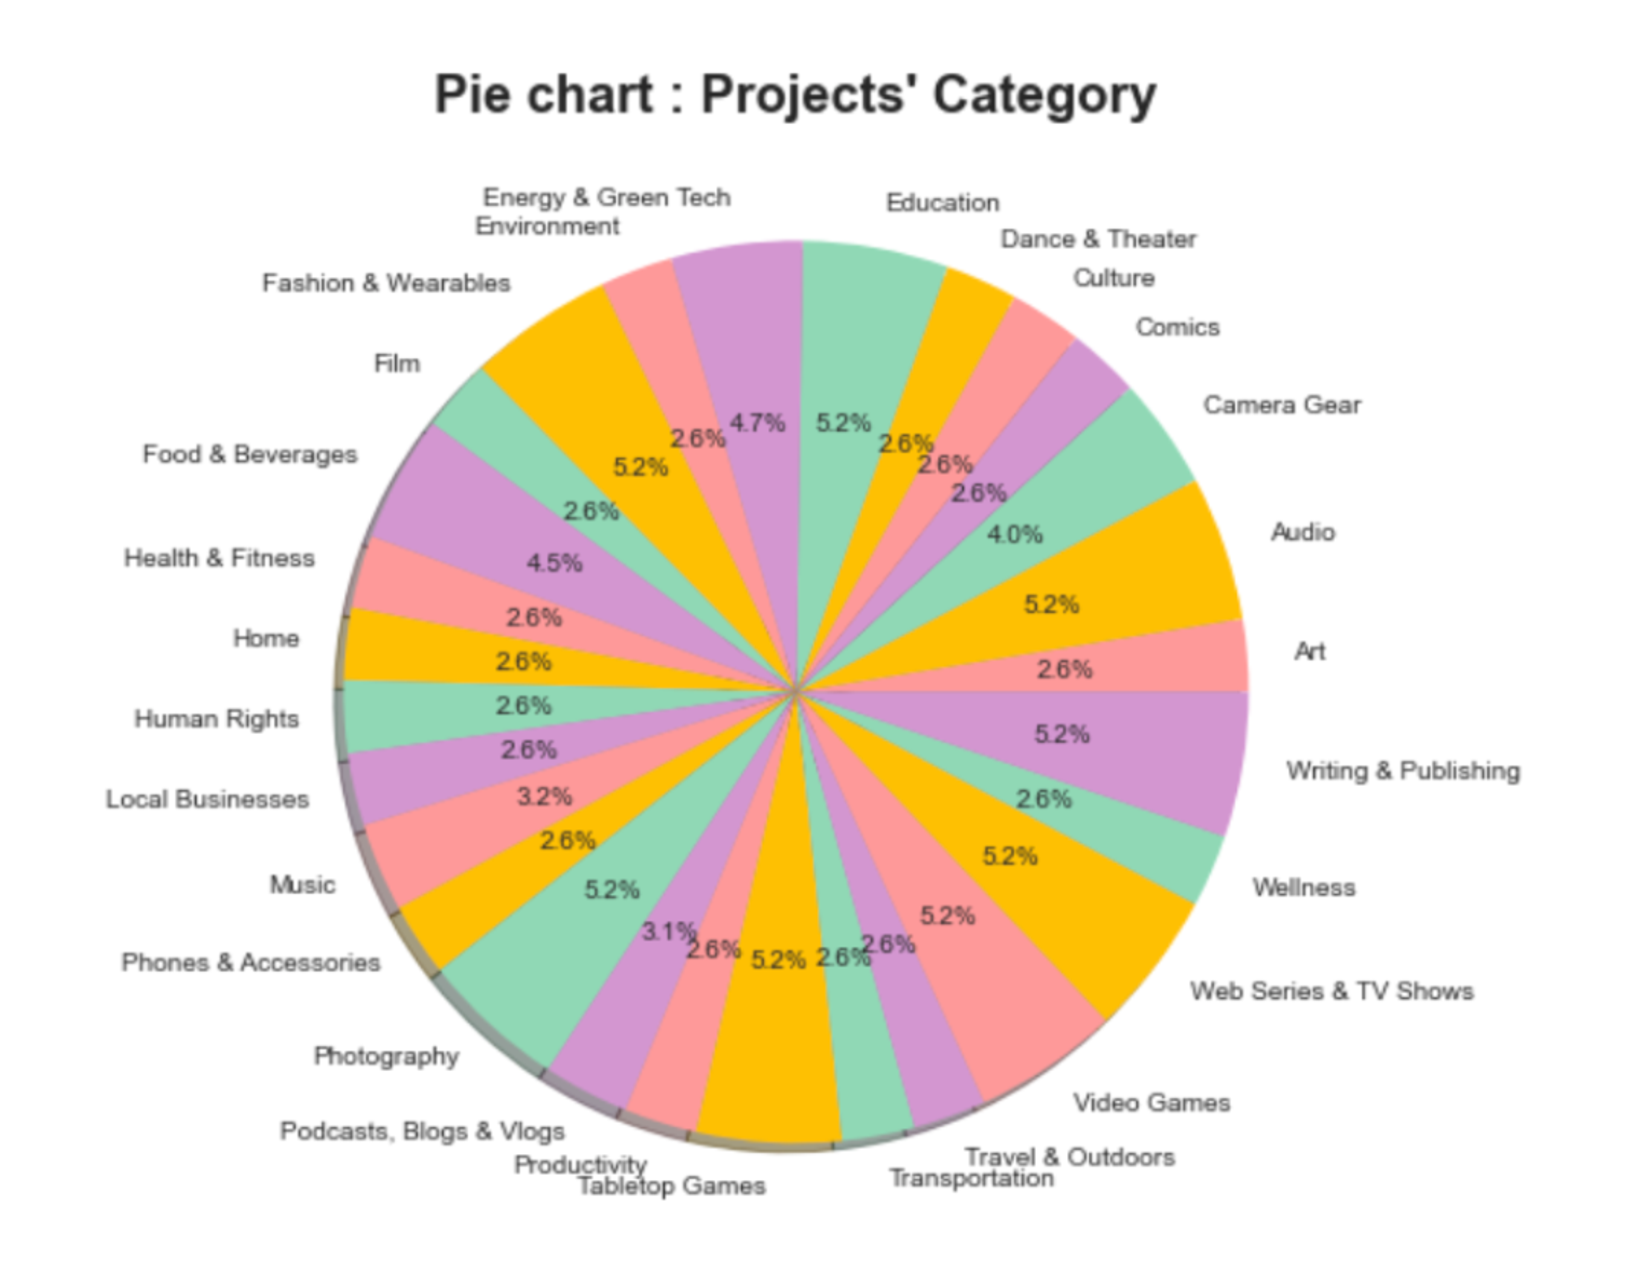
\includegraphics[width=8.5cm]{Figures/projects_pie_chart.pdf}
\vspace{-1em}
\caption{Pie chart showing type of Projects  and their percentages in Kickstarter"}
\vspace{-1em}
\label{fig:projects-pie-chart}
\end{figure} 